\documentclass[Lecture.tex]{subfiles}
\begin{document}
\section{3.1: Looking for Patterns with Scatterplots}
%\subsection{Constants}



\begin{frame}{Think-Pair-Share}
 For adults, there is a {\it positive association} between weight and height.  For used cars, there is a {\it negative association} between the age of the car and the selling price.  Explain what it means for two variables to have a positive association.  Explain what it means when two variables have a negative association.  What is an example of two variables that would have no association?
\end{frame}

\begin{frame}{Scatterplots}
\begin{defn}
\begin{itemize}
\item<1->
A {\it scatterplot} is a two-dimensional graph of the measurements for two numerical variables.
\item<2->
In a scatterplot, the response (dependent) variable is plotted on the vertical axis and the explanatory (independent) variable is plotted along the horizontal axis.
\end{itemize}
\end{defn}
\end{frame}

\begin{frame}{Scatterplots}
Questions to ask about a scatterplot:
\begin{itemize}
\item<1->
What is the {\it average} pattern? Is it a straight line or is it curved?
\item<2->
What is the direction of the pattern?
\item<3->
How much do individual points vary from the average pattern?
\item<4->
Are there any unusual data points?
\end{itemize}
\end{frame}

\begin{frame}{Associations}
\begin{defn}
\begin{itemize}
\item<1->
Two variables have a {\it positive association} when the values of one variable tend to increase as the values of the other variable increase.
\item<2->
Two variables have a {\it negative association} when the values of one variable tend to decrease as the values of the other variable increase.
\item<3->
Two variables have a {\it linear relationship} when the pattern of their relationship resembles a straight line.
\end{itemize}
\end{defn}
\end{frame}

\begin{frame}{Indicating Groups}
\begin{center}
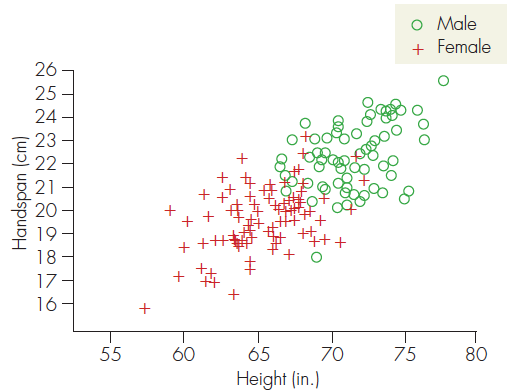
\includegraphics[scale=.4]{scatterplotgroups}
\end{center}
\end{frame}

\begin{frame}{Identifying Outliers}
\begin{center}
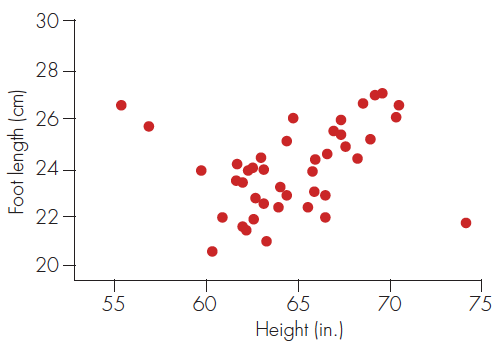
\includegraphics[scale=.4]{scatterplotoutliers}
\end{center}
\end{frame}












\end{document}
